\mysection{トランジスタの基本特性について}
トランジスタは小さな信号を大きな信号に増幅できる特性を持つ半導体素子である。
3つの電極は、E(エミッタ) C(コレクタ) B(ベース) で構成される。今回は、NPNトランジスタを扱う。

\begin{description}
  \setlength{\parskip}{0cm} % 段落間
  \setlength{\itemsep}{0cm} % 項目間
  \item[ゴール] $I_E$-$V_{BE}$ 特性、$I_C$-$I_B$ 特性、$I_C$-$V_{CE}$特性をLTspiceのシミュレーションで取得する。
  \item[キーワード] 直流電流増幅率、ダイオード特性
\end{description}

\mysubsection{演習手順}
\subsubsection{準備}
図\ref{tejun1}(a)の回路を作成する。
\begin{enumerate}
  \setlength{\parskip}{0cm} % 段落間
  \setlength{\itemsep}{0cm} % 項目間
  \item 「Component」→ 「npn」→ OK
  \item トランジスタを右クリック → 「Pick New Transistor」で「2SC1815」を選択しOK
  \item 電流源、電圧源を以下の図のように配置し、DCスイープを図\ref{tejun1}(b)のように設定
  \begin{figure}[htb]
    \begin{center}
    \subfigure[特性取得用]{	% 副題なし
    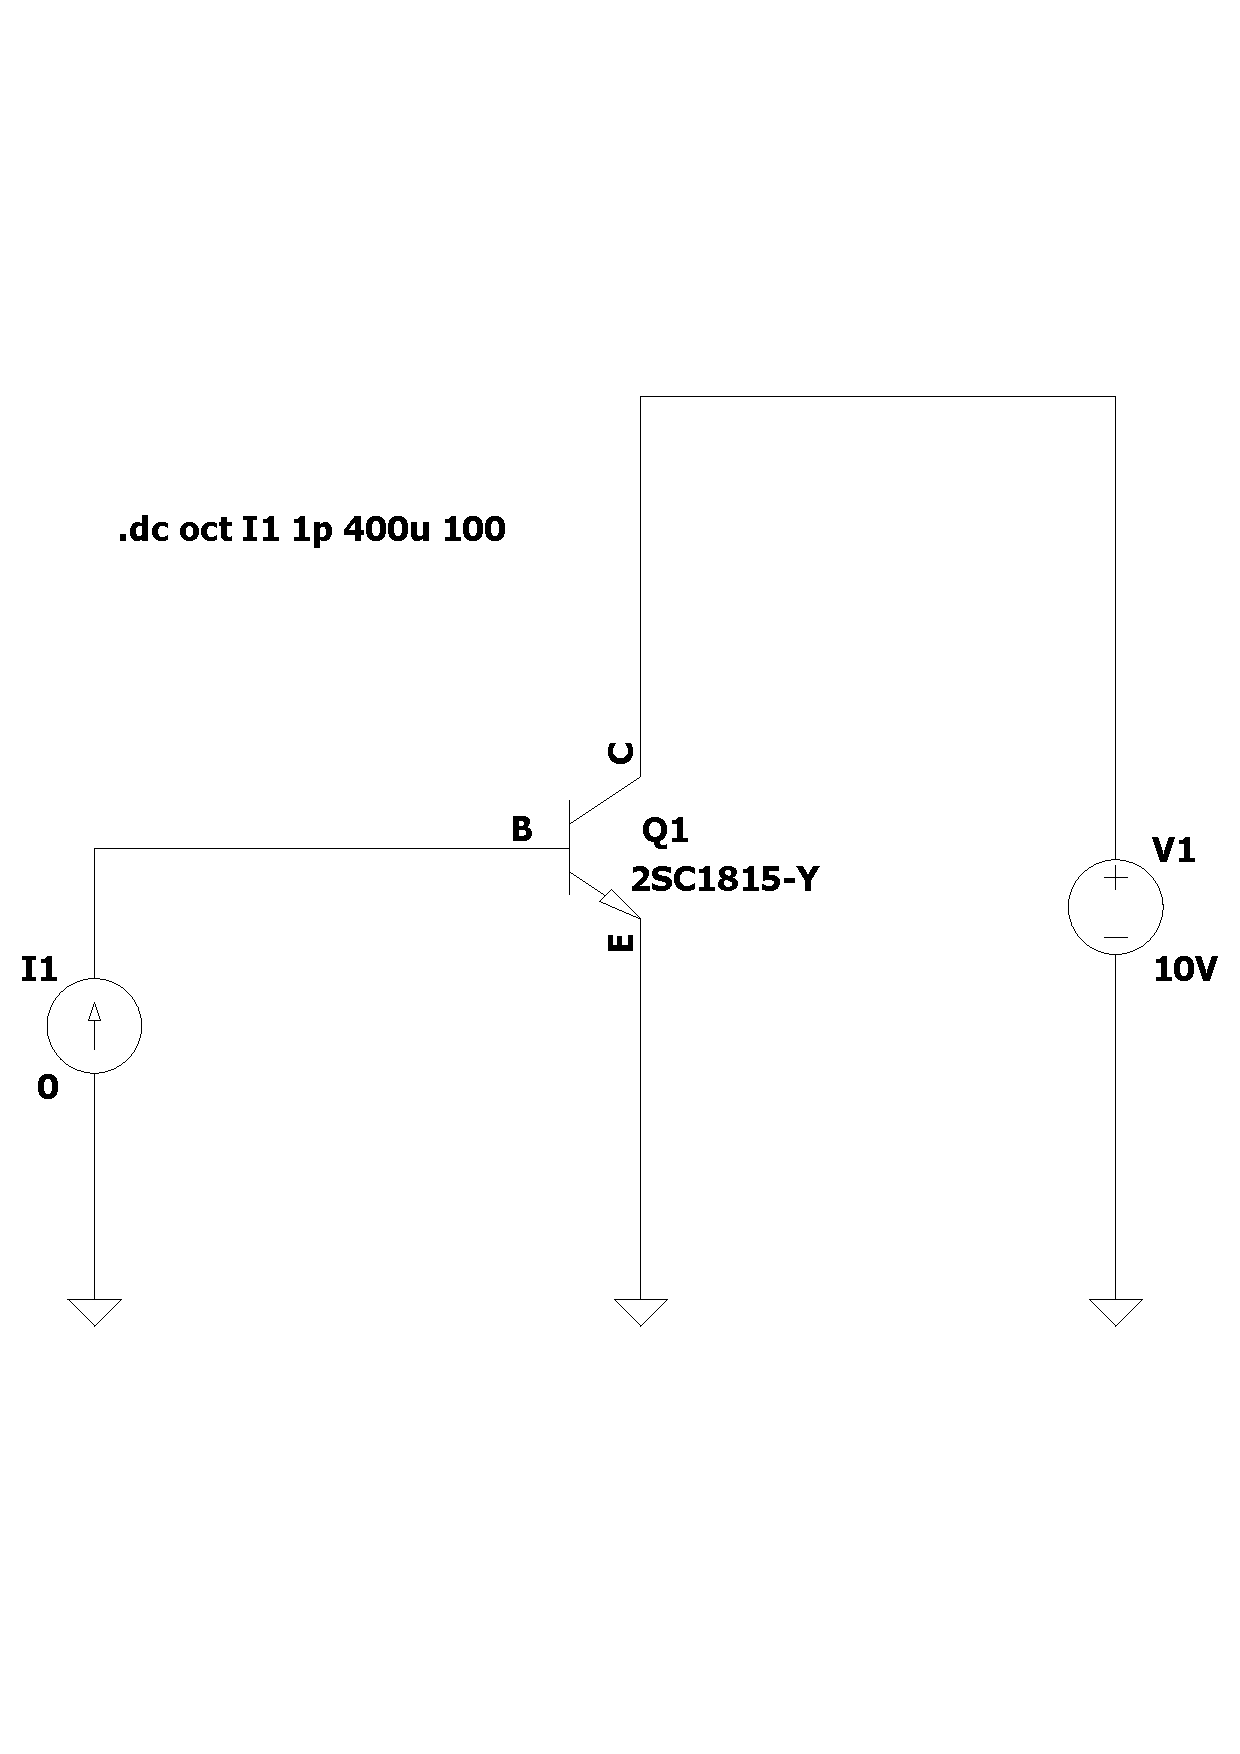
\includegraphics[width=.45\columnwidth]{img/25.pdf}
    }

    \subfigure[dcディレクティブタブ]{
    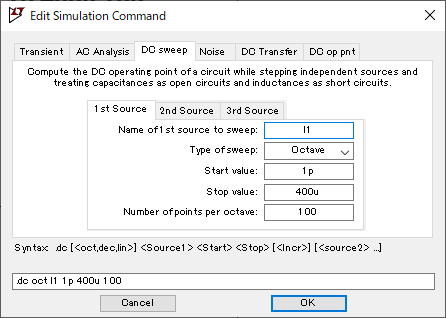
\includegraphics[width=.45\columnwidth]{img/26.png}
    }
    \subfigure[DCスイープ]{
    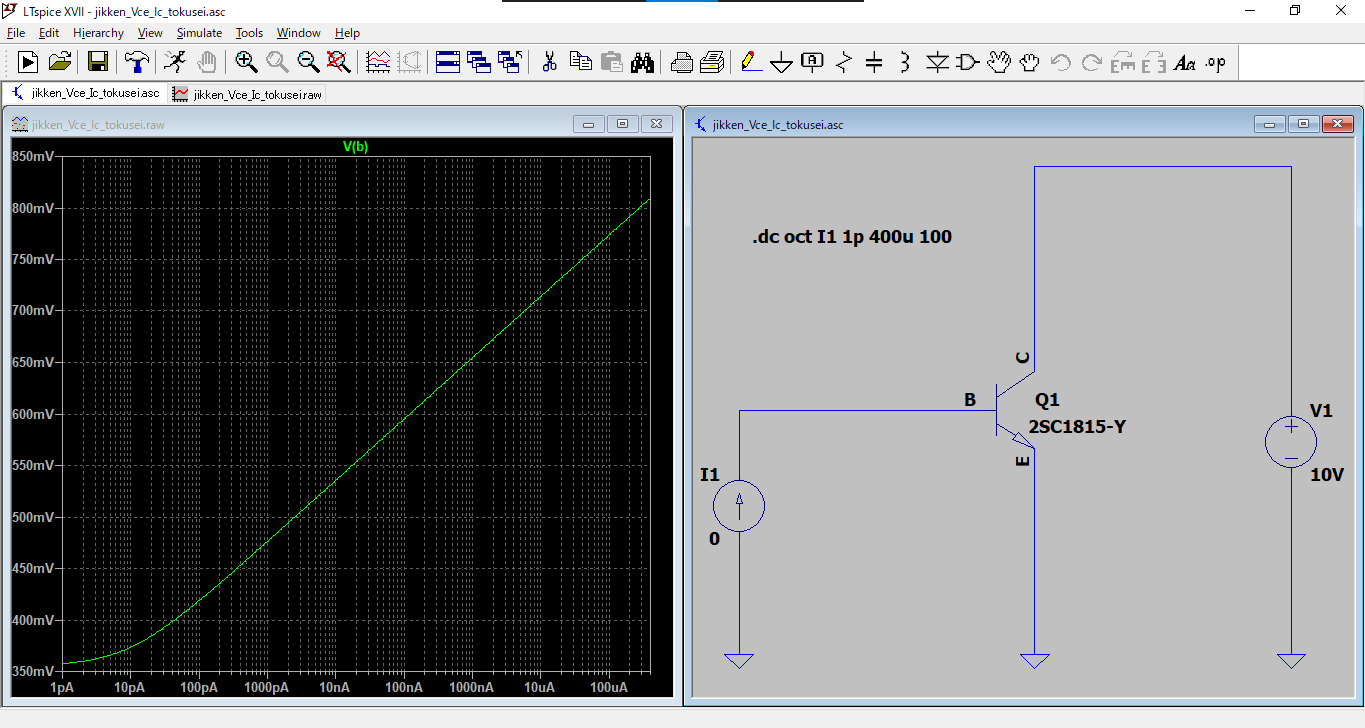
\includegraphics[width=.45\columnwidth]{img/27.png}
    }
    \caption{$I_E$-$V_{BE}$特性の取得方法} 
    \label{tejun1}
    \end{center}
  \end{figure}
  \item 「Run」ボタンをクリックして解析を実行する
  \item ベース電圧を測定する(プローブカーソルを合わせてクリックすると、図\ref{tejun1}(c)のような画面になる。)
\end{enumerate}
\vspace{-1\baselineskip}
\mysubsubsection{$I_E$-$V_{BE}$特性}
$I_E$-$V_{BE}$特性を図\ref{ie_vbe}に示す。
\begin{enumerate}
  \setlength{\parskip}{0cm} % 段落間
  \setlength{\itemsep}{0cm} % 項目間
  \item グラフの横軸にマウスカーソルを当てて定規カーソルで右クリック →「Horizontal Axis」→ 「Quantity Plotted」欄を "V(b)" に変更 → OKボタンクリックで終了。
  \item グラフの凡例のV(b)をクリック →「Expression Editor」→ 「Enter an algebraic expression to plot」を "-Ie(Q1)" に変更する。
  \item OKボタンをクリックして終了すると -Ie(Q1) vs V(b) のグラフが表示される。
  \item グラフの軸上で右クリックし、「Horizontal Axis」「Vertical Axis」「tick」を調整する。
  \begin{figure}[htb]
    \begin{center}
    \subfigure[$I_E$-$V_{BE}$特性(ダイオード特性)]{
    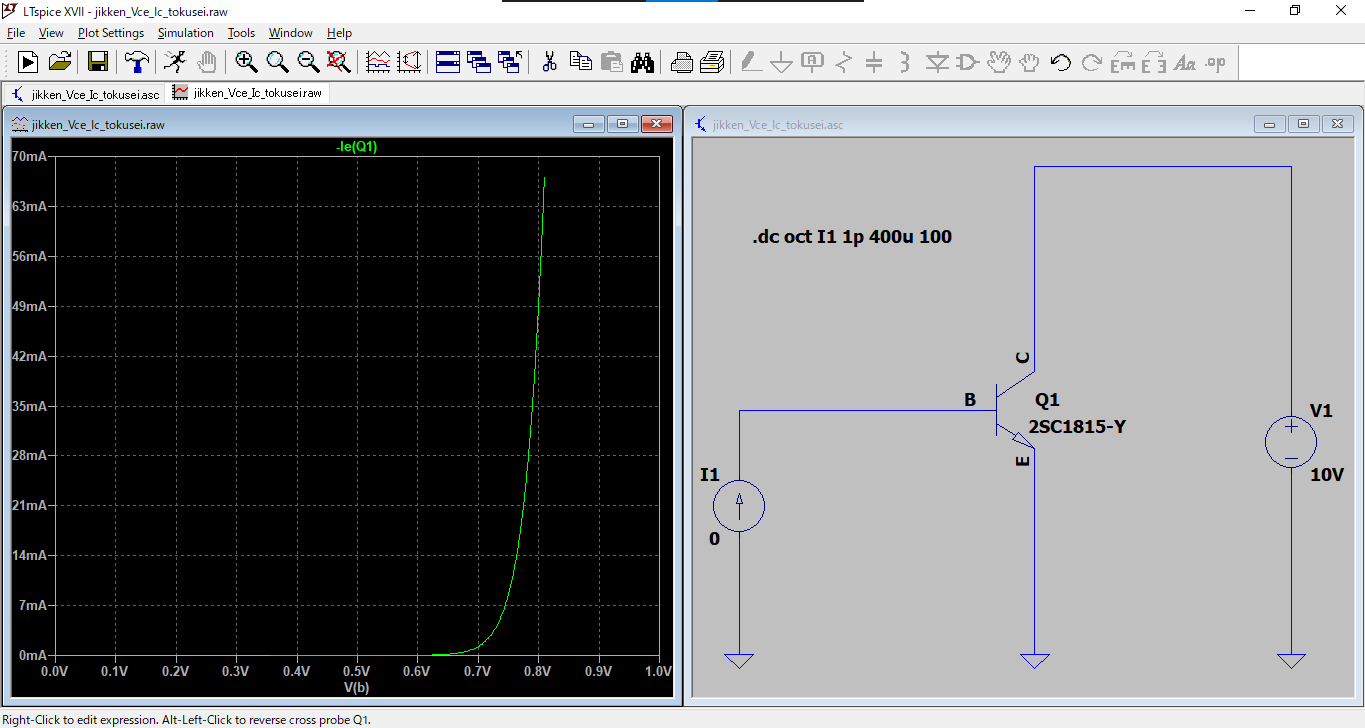
\includegraphics[width=.45\columnwidth]{img/28.png}
    }
    \subfigure[対数表示]{
    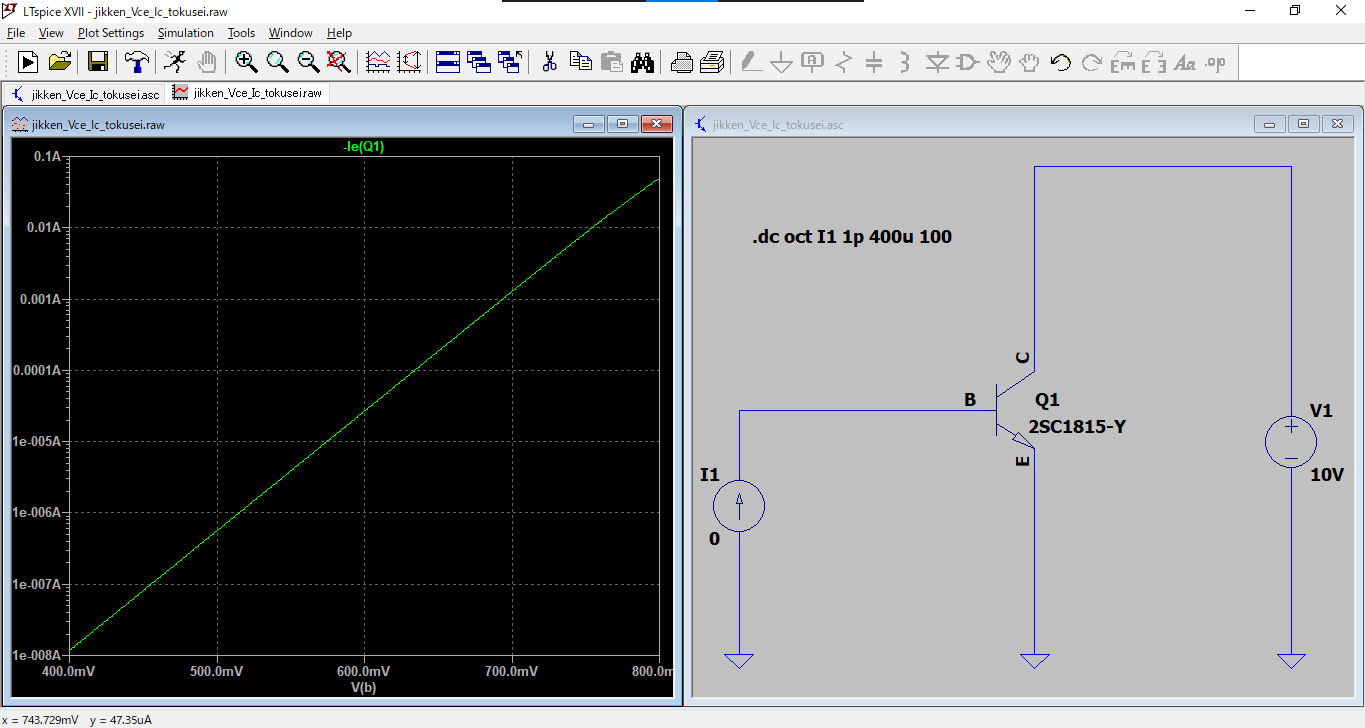
\includegraphics[width=.45\columnwidth]{img/29.png}
    }
    \caption{$I_E$-$V_{BE}$特性}
    \label{ie_vbe}
    \end{center}
  \end{figure}
  \item この特性を印刷するか画像で保存しておく。この回路図も保存しておく。
  \item 「Vertical Axis」→「Logarithmic」欄にチェック → OKと設定すると、片対数グラフでエミッタ電流が直線的に変化している。
\end{enumerate}

\begin{description}
  \setlength{\parskip}{0cm} % 段落間
  \setlength{\itemsep}{0cm} % 項目間
  \item[課題2] 2SC1815の$I_E$-$V_{BE}$特性をDCスイープにより取得して下さい。(用いた回路図とディレクティブを示すこと。図\ref{tejun1}(a)(c)、図\ref{ie_vbe}(a)(b)
  \item[任意課題4] 片対数グラフを用いて、$\frac{q}{kT}\log_{10}(e)$の値(理論値)と比較してください。\\
  カーソルを用いて傾きを求める。グラフ上部の凡例を右クリック →「Expression Editor」→「Attached Cursor」→ 1st \verb|&| 2nd を選んで十字カーソルを2個表示
\end{description}
\vspace{-0.5\baselineskip}
\mysubsubsection{$I_C$-$I_B$特性}
$I_C$-$I_B$特性を図\ref{ic_ib}に示す。「Edit Simulation Cmd」→ 「Edit Simulation Command」→「DC sweep」で以下のように設定しディレクティブを貼り付ける。
  \begin{figure}[htb]
    \begin{center}
    \subfigure[DCスイープ設定]{
    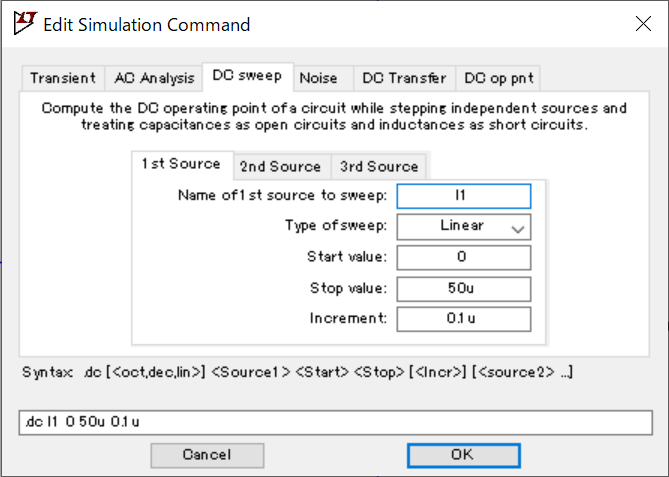
\includegraphics[width=.45\columnwidth]{img/30.png}
    }
    \subfigure[$I_C$-$I_B$特性]{
    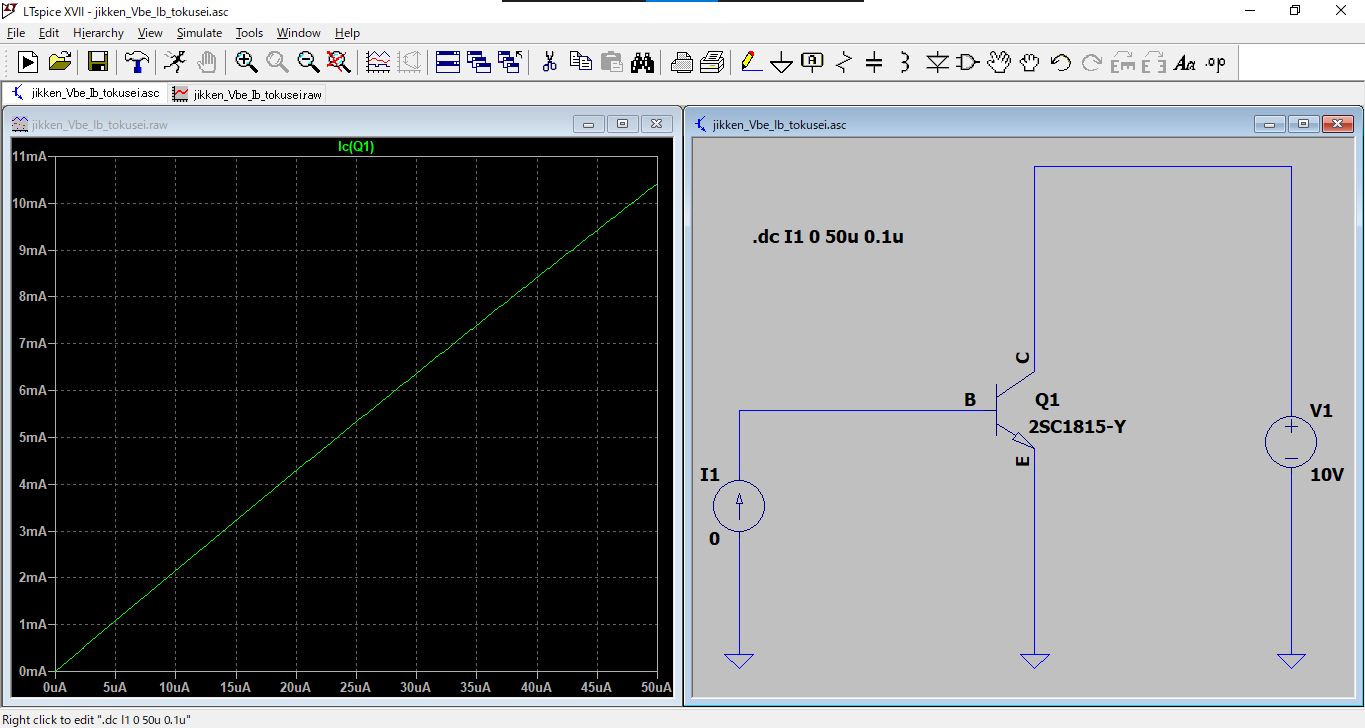
\includegraphics[width=.45\columnwidth]{img/31.png}
    }
    \caption{$I_C$-$I_B$特性}
    \label{ic_ib}
    \end{center}
  \end{figure}

\begin{description}
  \setlength{\parskip}{0cm} % 段落間
  \setlength{\itemsep}{0cm} % 項目間
  \item[課題3] 2SC1815の$I_C$-$I_B$特性をDCスイープにより取得して下さい。(用いた回路図とディレクティブを示すこと。図\ref{ic_ib}(a)(b)
  \item[任意課題5] $I_C-I_B$ 特性を用いてエミッタ交流電流増幅率と接地直流電流増幅率を求めて下さい。その値を直流電流増幅率と比較して下さい。
  \item[交流電流増幅率] 特性曲線の1点で、ベース電流とコレクタ電流の増幅率を求める。
  \item[直流電流増幅率] 特性曲線の2点で、ベース電流とコレクタ電流の増幅率を求める。
\end{description}
\vspace{-1\baselineskip}
\mysubsubsection{$I_C$-$V_{CE}$特性}
$I_C$-$V_{CE}$特性を取得するためのopディレクティブの設定を図\ref{ic_vce_op}、$I_C$-$V_{CE}$特性を図\ref{ic_vce}に示す。
\begin{enumerate}
  \setlength{\parskip}{0cm} % 段落間
  \setlength{\itemsep}{0cm} % 項目間
  \item $I_1$をパラメータとして設定する。$I_1$を右クリックして \verb|"{IB}"| と入力する。
  \item spiceディレクティブを設定
    \begin{itemize}
      \setlength{\parskip}{0cm} % 段落間
      \setlength{\itemsep}{0cm} % 項目間
      \item 「SPICE Directive」(.op) → 「Edit Text on the Schematic」→ 入力欄で右クリック「Help me Edit」→ 「.step Command」→ 「.step Statement Editor」にSPICEディレクティブを書き込む → OK
      \item \verb|.step param IB list 10u 15u 20u 25u 30u 35u 40u 45u 50u| と入力

    \begin{figure}[htb]
      \begin{center}

      \subfigure[$I_C$-$V_{CE}$特性]{	% 副題なし
      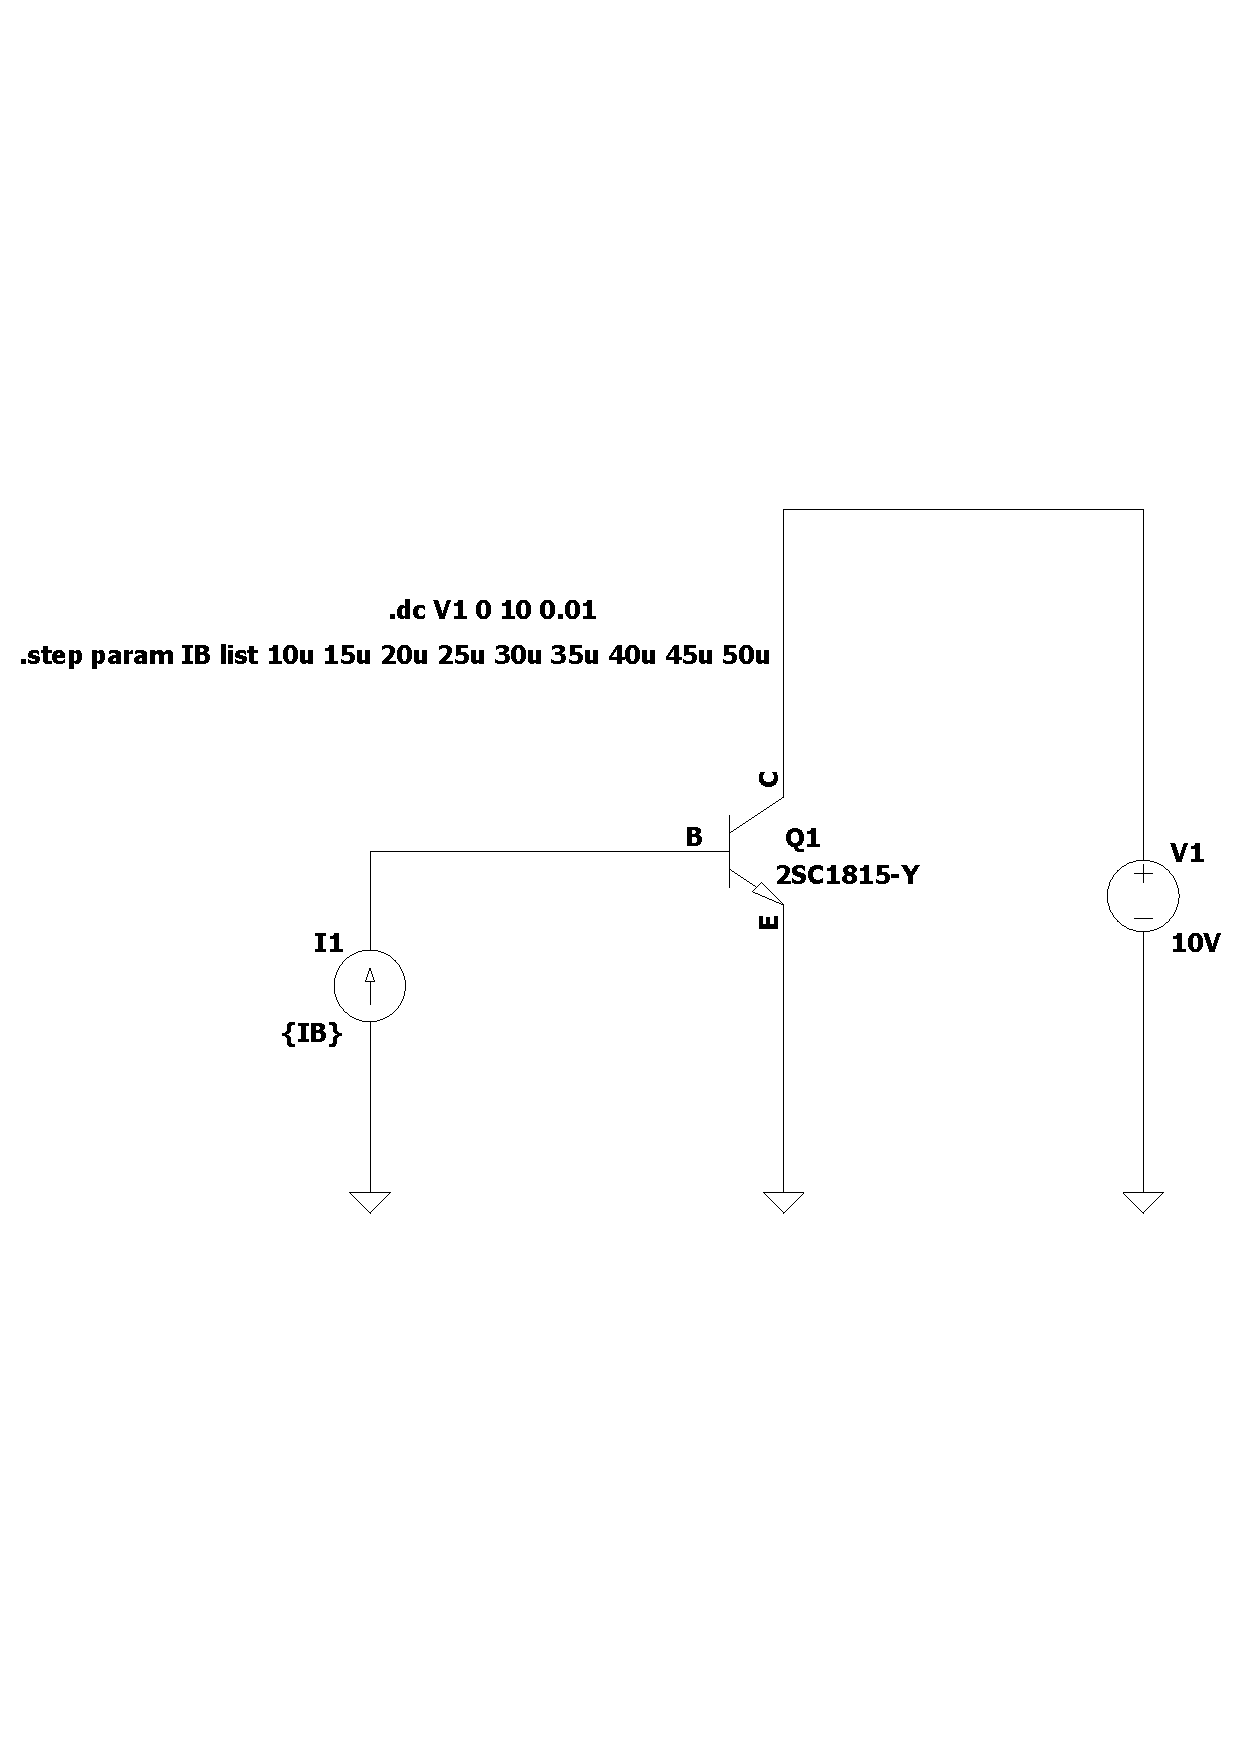
\includegraphics[width=.7\columnwidth]{img/32.pdf}
      }
      \subfigure[.op ディレクティブ]{
      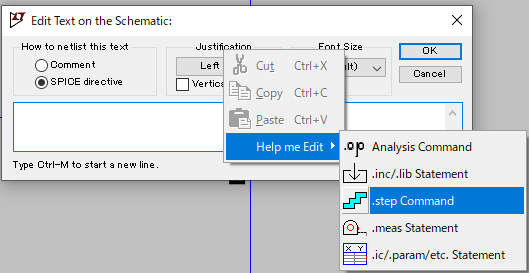
\includegraphics[width=.45\columnwidth]{img/33.png}
      }
      \subfigure[stepパラメータの設定]{
      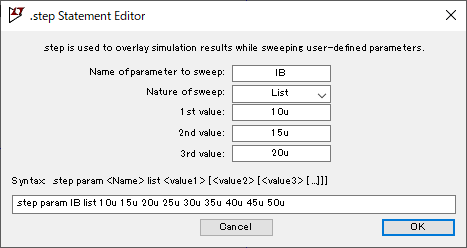
\includegraphics[width=.45\columnwidth]{img/34.png}
      }
      \caption{.op ディレクティブの設定}
      \label{ic_vce_op}
      \end{center}
    \end{figure}
  \end{itemize}
  \item DCスイープの設定
  \begin{itemize}
    \setlength{\parskip}{0cm} % 段落間
    \setlength{\itemsep}{0cm} % 項目間
    \item \verb|.dc V1 0 10 0.01|
    \item 「Run」をクリックし、$I_C$をプローブで測る。
  \end{itemize}
  \begin{figure}[htb]
    \begin{center}
    \subfigure[$I_C$-$V_{CE}$特性の.opディレクティブ実行結果]{
    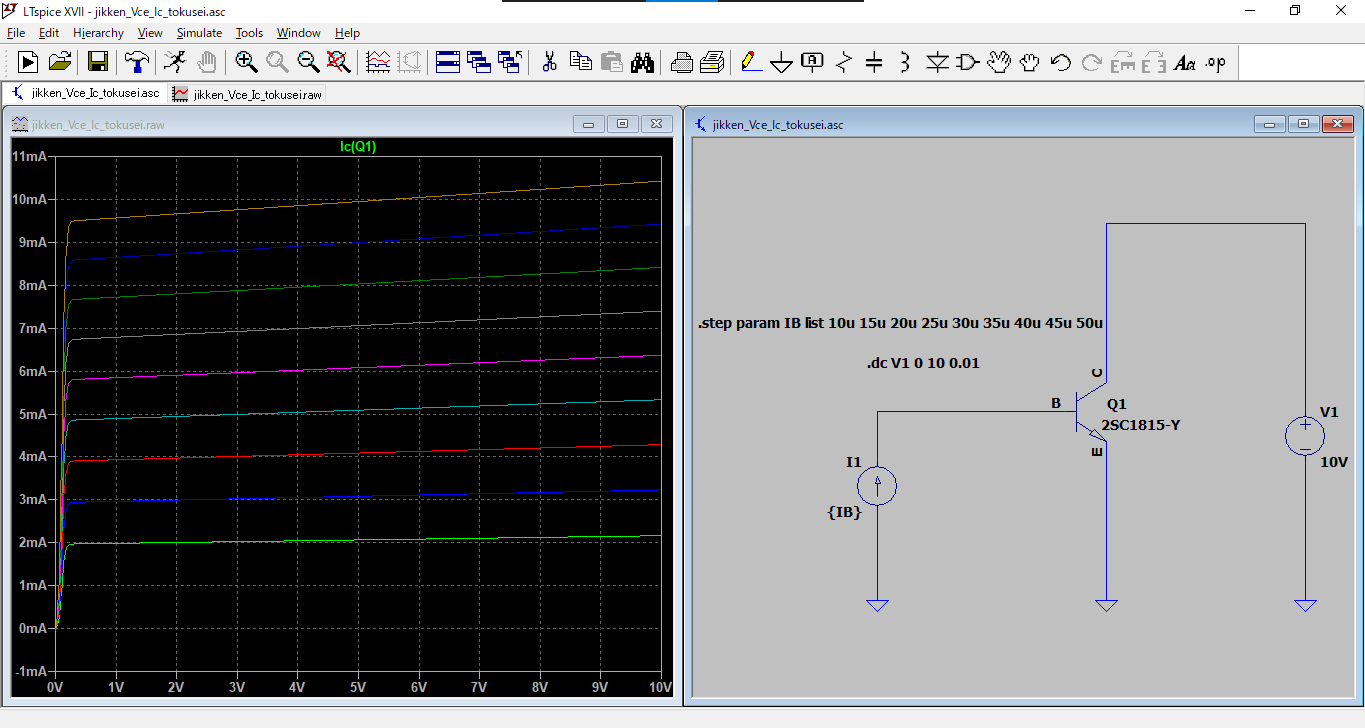
\includegraphics[width=.55\columnwidth]{img/35.png}
    }
    \subfigure[$I_C$-$V_{CE}$特性]{
    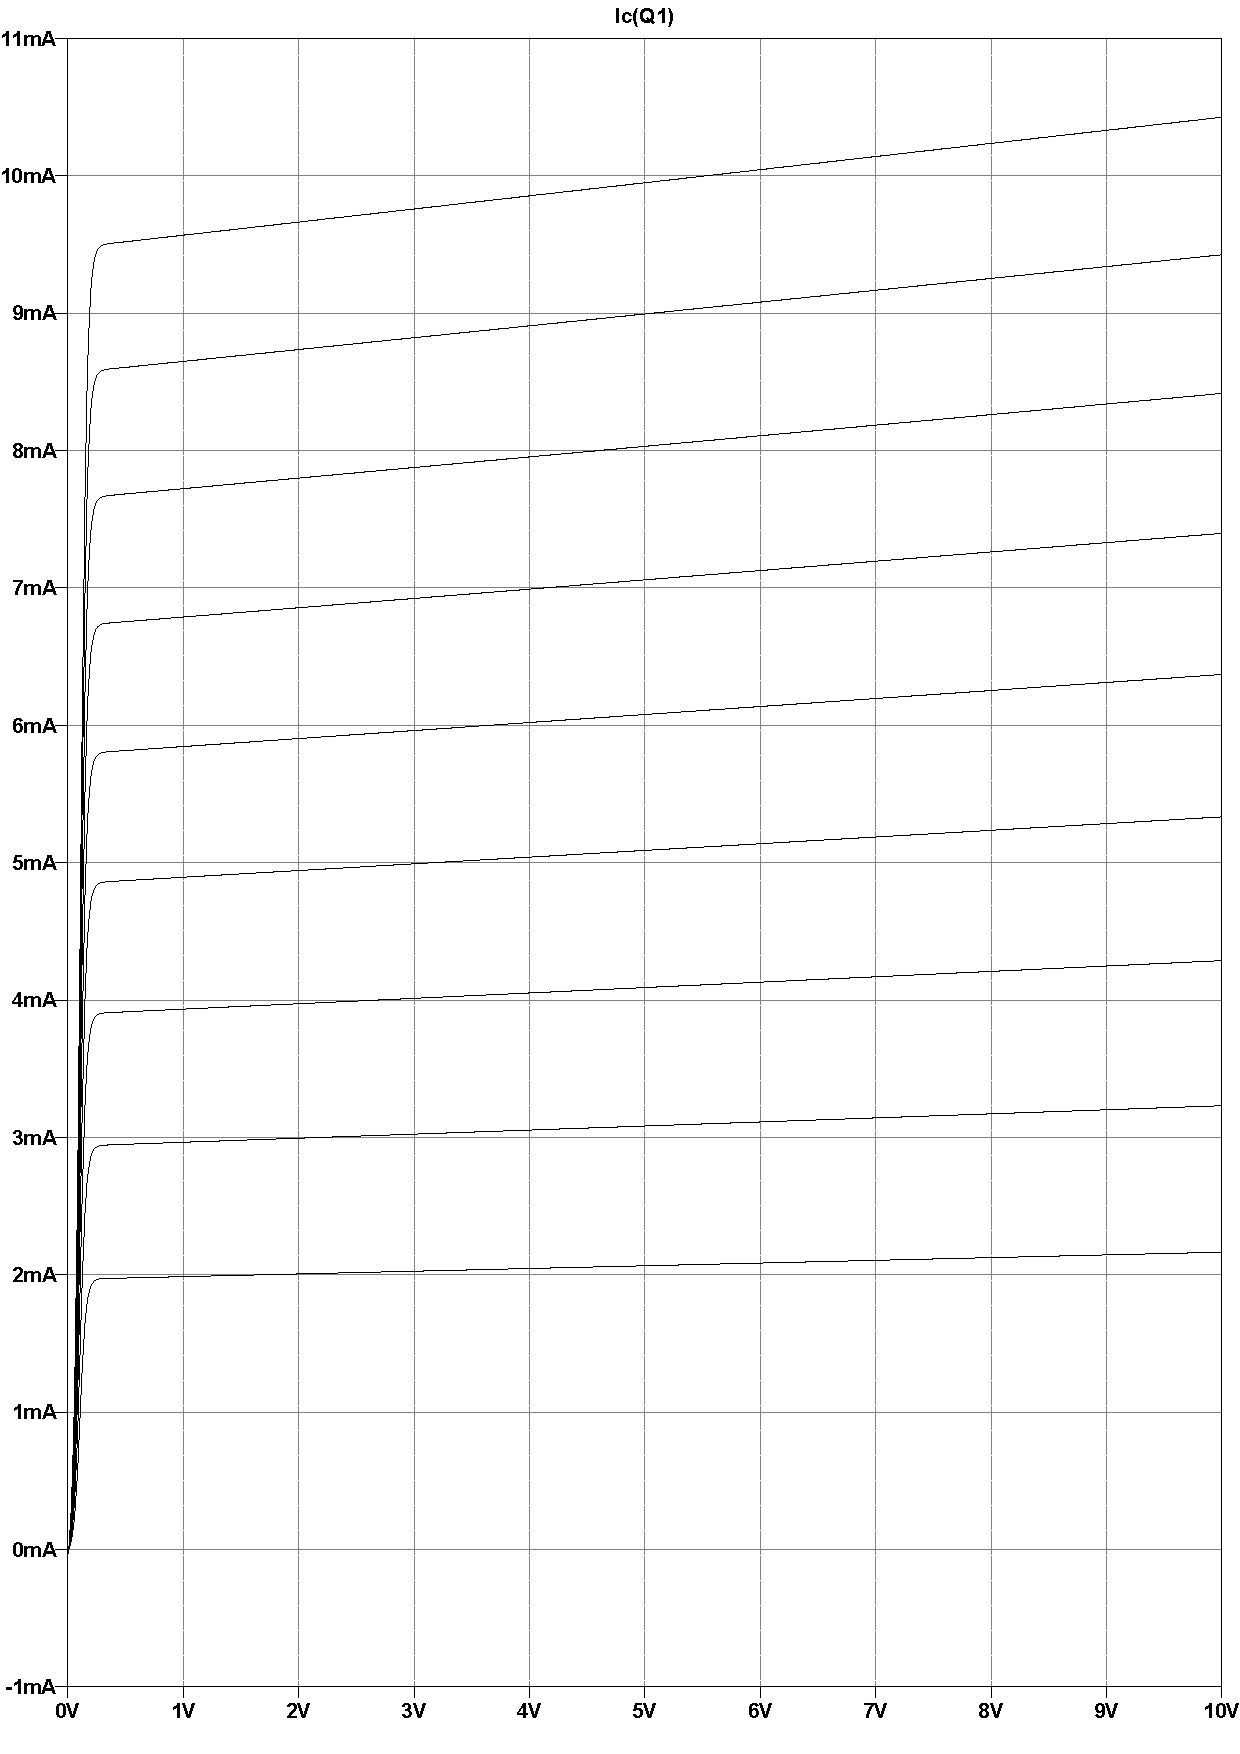
\includegraphics[width=.35\columnwidth]{img/36.pdf}
    }
    \caption{$I_{CE}$-$V_{CE}$特性}
    \label{ic_vce}
    \end{center}
  \end{figure}
    \item この特性を印刷するか画像で保存しておく。
    \begin{description}
      \setlength{\parskip}{0cm} % 段落間
      \setlength{\itemsep}{0cm} % 項目間
      \item[課題4] 2SC1815の$I_C$-$V_{CE}$ 特性をSPICEディレクティブを用いて取得して下さい。(用いた回路図とディレクティブを示すこと。図\ref{ic_vce_op}(a)、図\ref{ic_vce}(a)(b))
      \item[任意課題6] $I_C$-$V_{CE}$ 特性から、入力信号トランジスタの増幅回路を設計するための$V_{CE}$の領域は何 V \verb|~| 何 V が良いでしょうか?
    \end{description}
\end{enumerate}